\begin{frame}
\frametitle{About This Work...}

\emph{Spatiotemporal Cleansing for Indoor RFID Tracking Data}.~\cite{baba2013spatiotemporal} \\
A.I.~Baba, H.~Lu, X.~Xie, T.B.~Pedersen\\~\\

\begin{itemize}
  \item Published at \emph{MDM' 2013}.
  \item Focused on two quality aspects in raw indoor RFID data, temporal redundancy and spatial ambiguity.
  \item Investigated the spatiotemporal characteristics of indoor spaces as well as RFID reader deployment to be exploited in cleansing.
\end{itemize}

\end{frame}

%------------------------------------------------

\begin{frame}
\frametitle{Motivation}

\begin{itemize}
  \item Effective RFID tracking data management is expected to support various applications.
  \begin{sitemize}
    \item range from monitoring to analysis of indoor moving objects
    \item RFID reader reports the object's presence to the database that manages the object positions
  \end{sitemize}
  \item However, noises and errors abound in raw data.
  \begin{sitemize}
    \item radio frequency waves are not steady and therefore the detection range may change from time to time
    \item such dirtiness hinders the progress of applying meaningful high level application.
  \end{sitemize}
  \item Cleansing RFID data is therefore needed.
\end{itemize}

\end{frame}

%------------------------------------------------

\begin{frame}
\frametitle{Dirtiness in Indoor RFID Tracking Data}

\textrm{An RFID reader report $(readerID, objectID, time)$ means the object identified by $objectID$ is seen by the reader identified by $readerID$ at time point $time$}.\\~\\

\conceptbf{Temporal Redundancy}~~~~A tagged object can be read many times by the same reader within a short period, depending on the sampling frequency configured for a reader.\\~\\

\conceptbf{Spatial Ambiguity}~~~~A tagged object can be read by multiple readers simultaneously. This may result from the unexpected change of the detection range of a reader nearby.

\end{frame}

%------------------------------------------------

\begin{frame}
\frametitle{Dirtiness in Indoor RFID Tracking Data}

\begin{figure}[tb]
  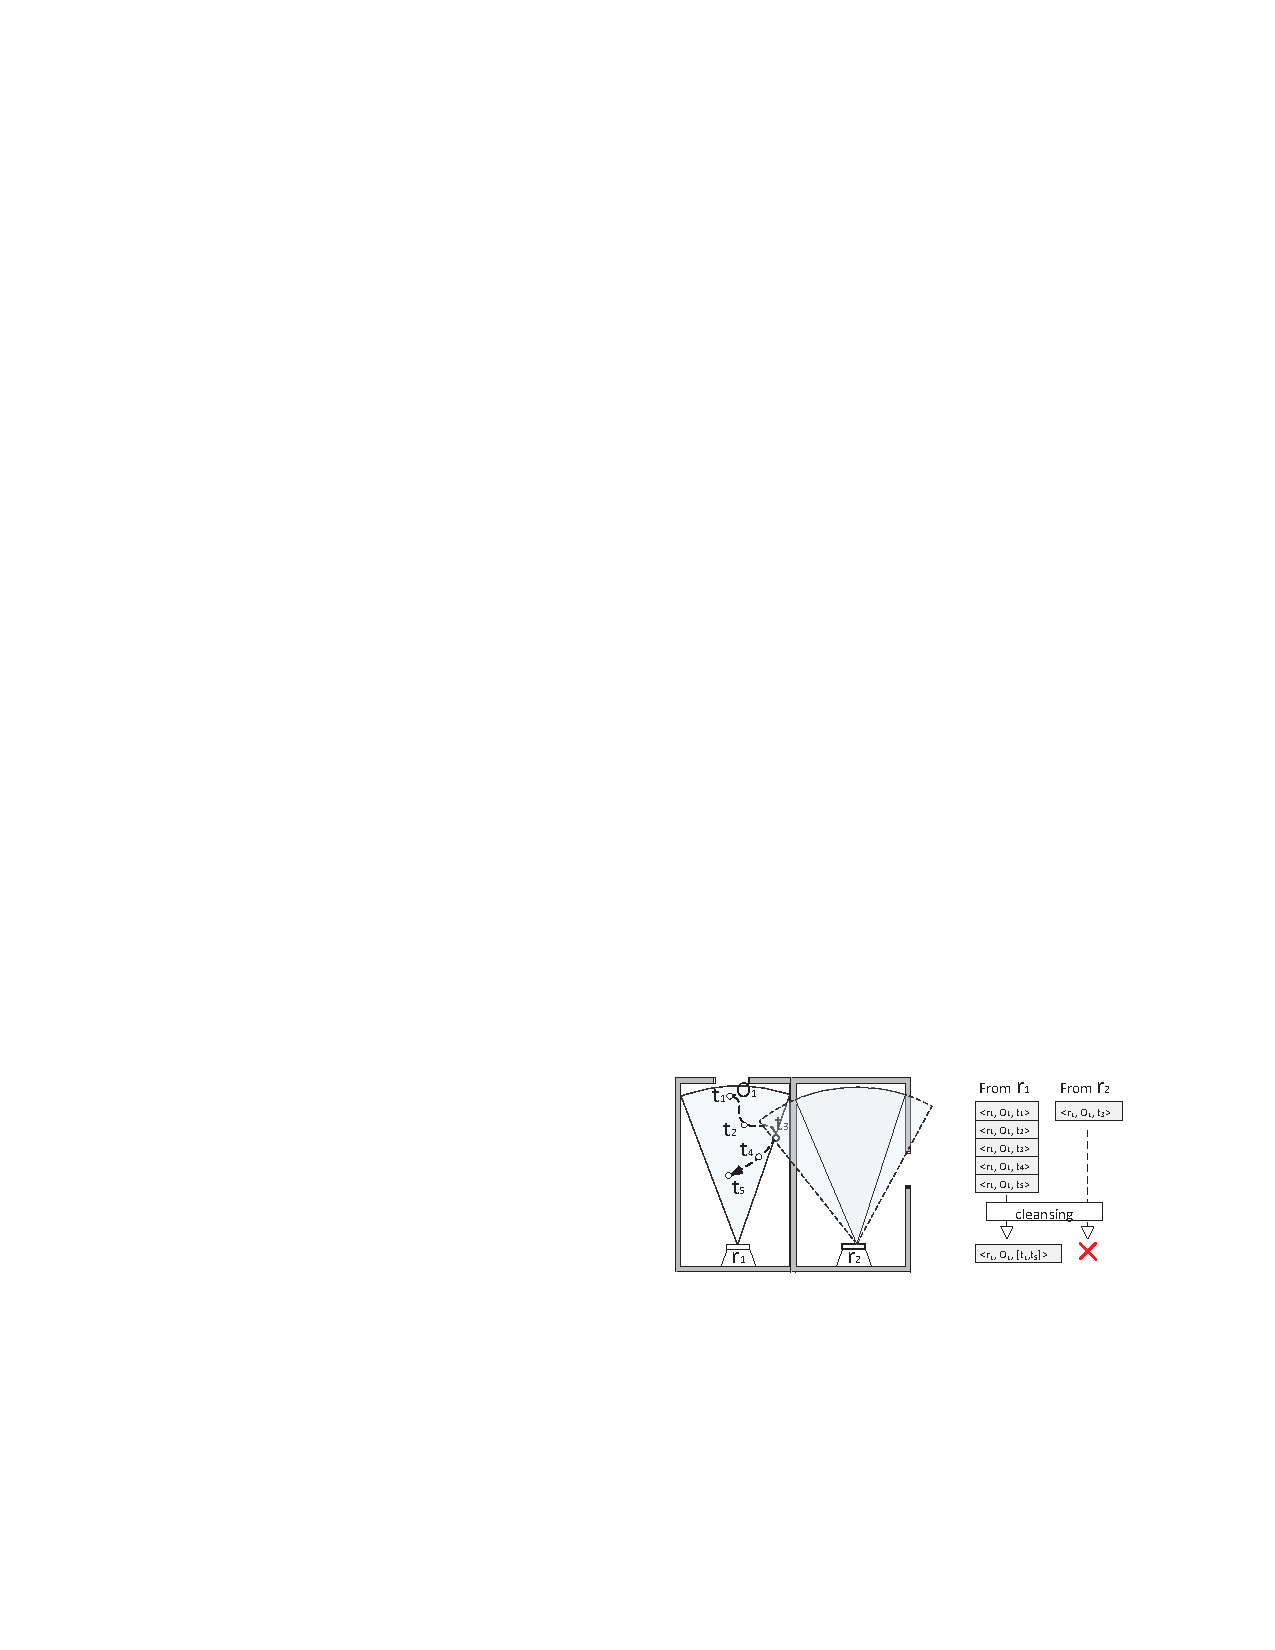
\includegraphics[width=0.6\columnwidth]{figures/3-2/3-2-1.pdf}
\end{figure}

\vspace{-15pt}
\begin{columns}

  \column{0.5\textwidth}
  \begin{example}
    \ssize{
    Two readers $r_1$, $r_2$ in two rooms respectively. Object $O_1$ moves in the left room from time point $t_1$ to time point $t_5$, which yields five reports by $r_1$ as the trajectory is within $r_1$'s detection range. If times points are very close to each other, the five reports can be compressed into a single tuple $\langle r_1, O_1, [t_1,t_5] \rangle$.
    }
  \end{example}

  \column{0.5\textwidth}
  \begin{example}
    \ssize{
    At time point $t_3$, object $O_1$ is detected by both readers. This is due to the unexpected expansion of $r_2$'s detection range. Consequently, from the RFID data, $O_1$ seems to be in both rooms at same time $t_3$. Thus spatial ambiguity is caused. By considering such spatiotemporal constraints, our cleansing technique is able to remove spatial ambiguous reports such as $\langle r_2, O_1, t_3 \rangle$.
    }
  \end{example}

\end{columns}

\end{frame}

%------------------------------------------------

\begin{frame}
\frametitle{Raw Readings Table (RRT)}

\begin{columns}[c]

  \column{0.55\textwidth}
  \begin{figure}[tb]
    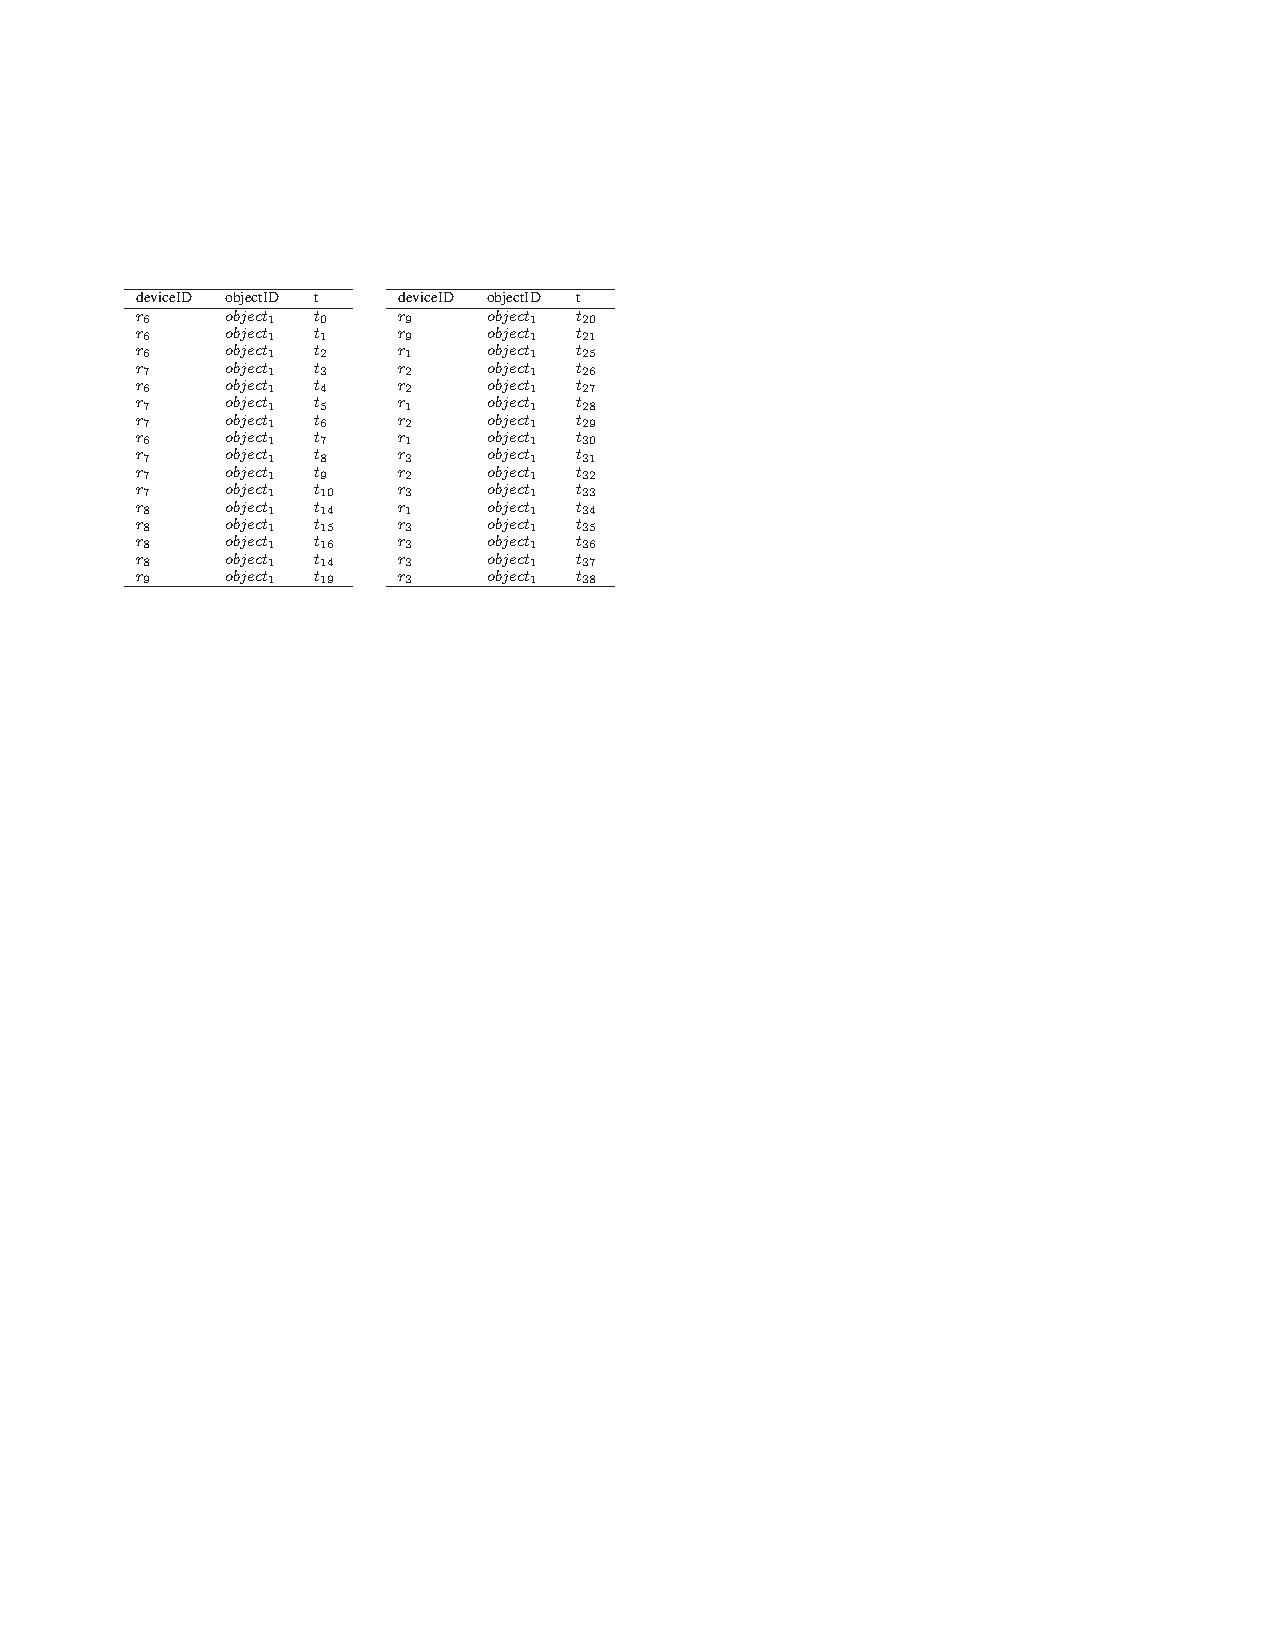
\includegraphics[width=\columnwidth]{figures/3-2/3-2-2.pdf}
  \end{figure}

  \column{0.45\textwidth}
  \begin{sitemize}
    \item each raw reading is in the format of $(deviceID, objectID, t)$, which means that the object identified by $objectID$ is detected by the device identified by $deviceID$ at time $t$.
    \item usually the detection range of a positioning device is a circular region with a pre-specified radius, a positioning device continuously detects objects that are in its range, with the frequency determined by its sampling rate.
  \end{sitemize}

\end{columns}

\end{frame}

%------------------------------------------------

\begin{frame}
\frametitle{Compared with Graph Based Indoor Tracking~\cite{DBLP:conf/mdm/JensenLY09}}

This paper distinguishes itself from the work~\cite{DBLP:conf/mdm/JensenLY09} introduced in Section 2.1:

\begin{itemize}
  \item This paper considers the overlapping between different positioning devices, whereas work~\cite{DBLP:conf/mdm/JensenLY09} assumes that devices do not overlap.
  \item This paper is intended to decide where an object really is when is is seen by multiple devices, whereas work~\cite{DBLP:conf/mdm/JensenLY09} focuses on tracking the object when it is not seen by any devices.
  \item In order to support data cleansing, this paper proposes a \emph{Distance-Aware Graph} different from the \emph{Deployment Graph} introduced in Section 2.
\end{itemize}

\end{frame}

%------------------------------------------------

\begin{frame}
\frametitle{Notations}

\begin{figure}[tb]
  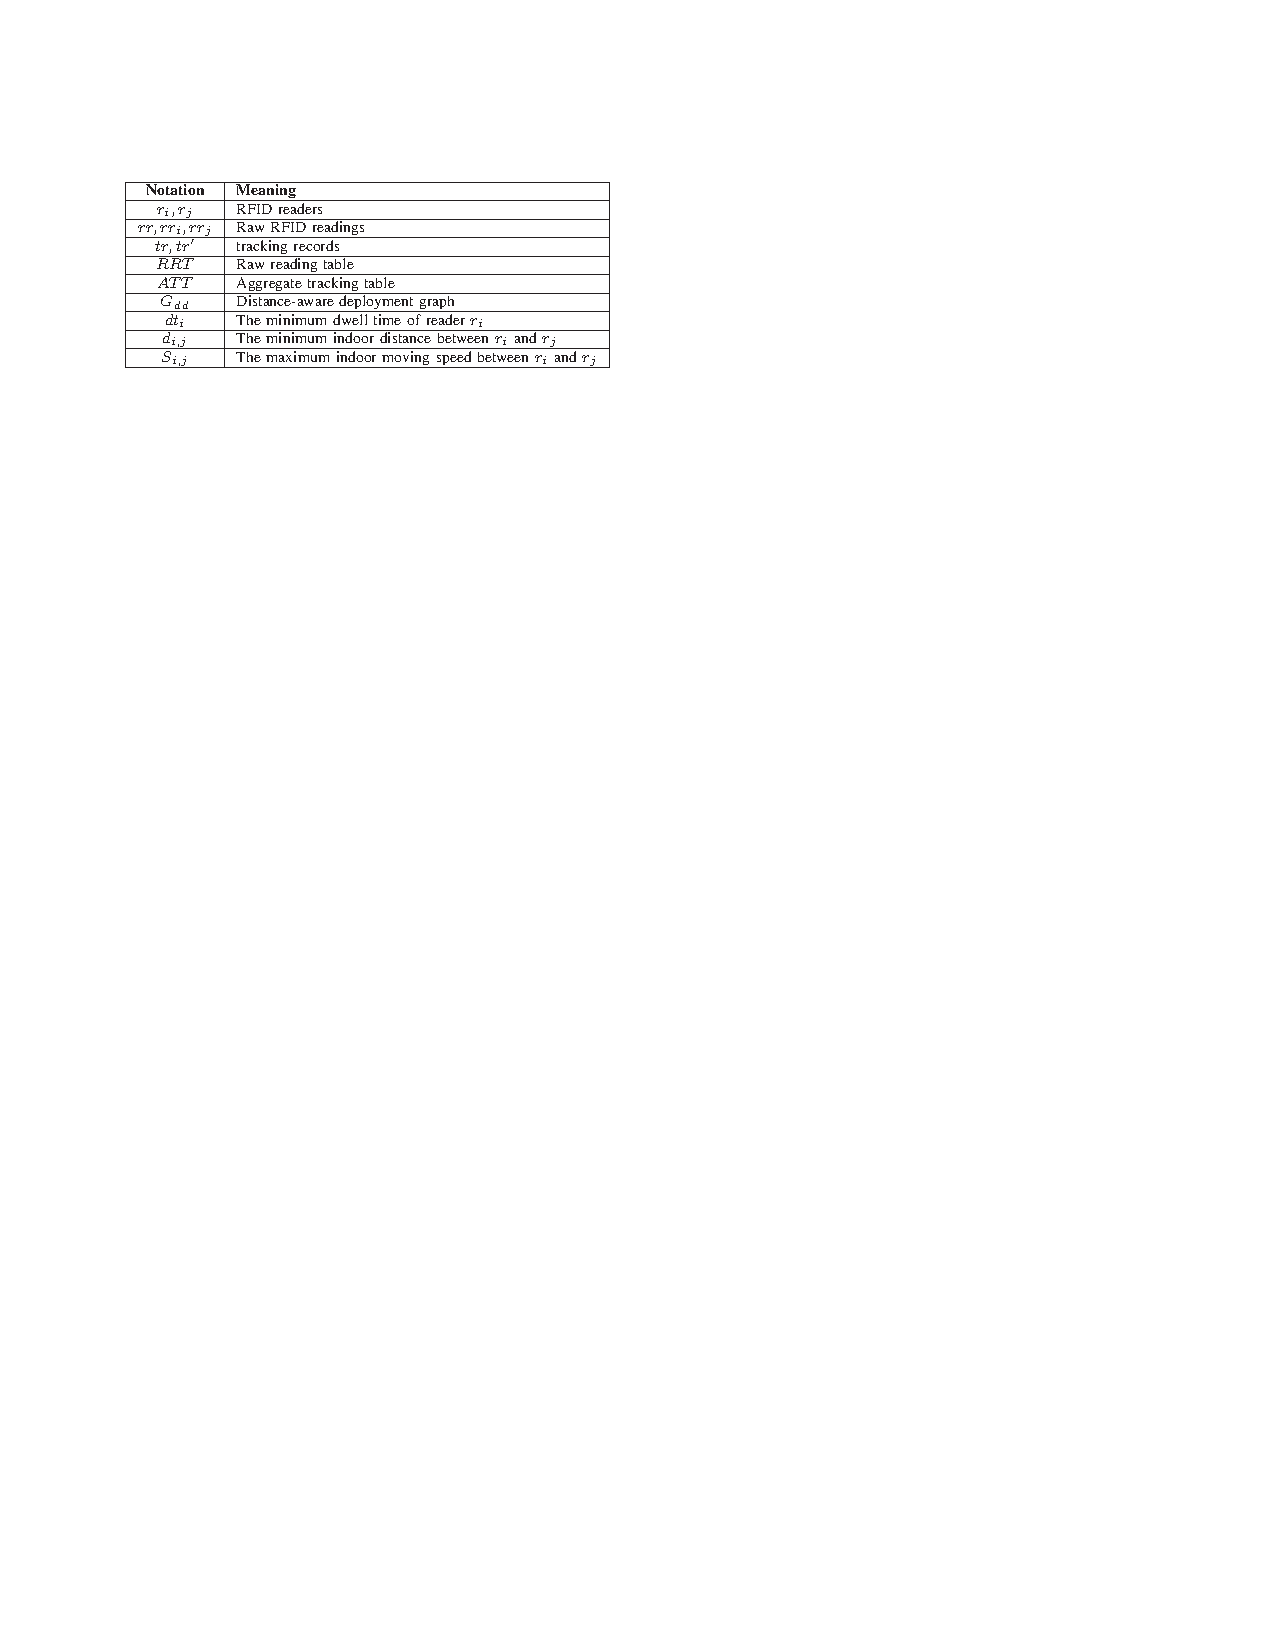
\includegraphics[width=\columnwidth]{figures/3-2/3-2-3.pdf}
\end{figure}

\end{frame}

%------------------------------------------------

\begin{frame}
\frametitle{Definitions and Tasks}

\begin{definition}[Temporal Redundant Readings]
  Two raw readings $rr_i$ and $rr_j$ are temporal redundant readings if $|rr_i.t - rr_j.t| \leq \tau$, $rr_i.deviceID = rr_j.deviceID$ and $rr_i.objectID = rr_j.objectID$, where $\tau$ is an application-specific threshold.
\end{definition}

\begin{definition}[Tracking Record]
  Given a series of temporal redundant readings $rr_1, ..., rr_k$, a tracking record $tr$ is a temporal aggregation of them. Formally, $tr$ is in the format $(deviceID, objectID, t_s, t_e)$, where $tr.deviceID = rr_i.deviceID$, $tr.objectID = rr_i.objectID$, $tr.t_s = rr_1.t$ and $tr.t_e = tt_k.t$ for $1 \leq i \leq k$.
\end{definition}

\end{frame}

%------------------------------------------------

\begin{frame}
\frametitle{Definitions and Tasks}

\begin{definition}[Spatial Ambiguous Tracking Records]
  Two tracking records $tr'$ and $tr$ are spatial ambiguous if $tr'.deviceID \neq tr.deviceID$ and $tr'.objectID = tr.objectID$, if $tr'.[t_s, t_e] \cap tr.[t_s, t_e] \neq \varnothing $, or if $tr.t_s - tr'.t_e \leq min\_tt$, where $min\_tt$ is the minimum travelling time for an object to move from $tr'$'s device to $tr$'s device.
\end{definition}

\end{frame}

%------------------------------------------------

\begin{frame}
\frametitle{Definitions and Tasks}

\begin{block}{Task (Temporal Redundancy Elimination)}
  This task is to aggregate raw readings into more meaningful tracking records. This way is expected to significantly reduce the data size without any information loss.
\end{block}

\begin{block}{Task (Spatial Ambiguity Reduction)}
  Given a large set of tracking records, this task is to identify spatial ambiguous tracking records and reduce such spatial ambiguities by referring to the spatiotemporal constrains imposed by the positioning device deployment as well as the indoor topology.
\end{block}

\textrm{these two tasks together are called \conceptbf{spatiotemporal data cleansing}}.

\end{frame}

%------------------------------------------------

\begin{frame}
\frametitle{Overview of Spatiotemporal Data Cleansing}

\begin{figure}[tb]
  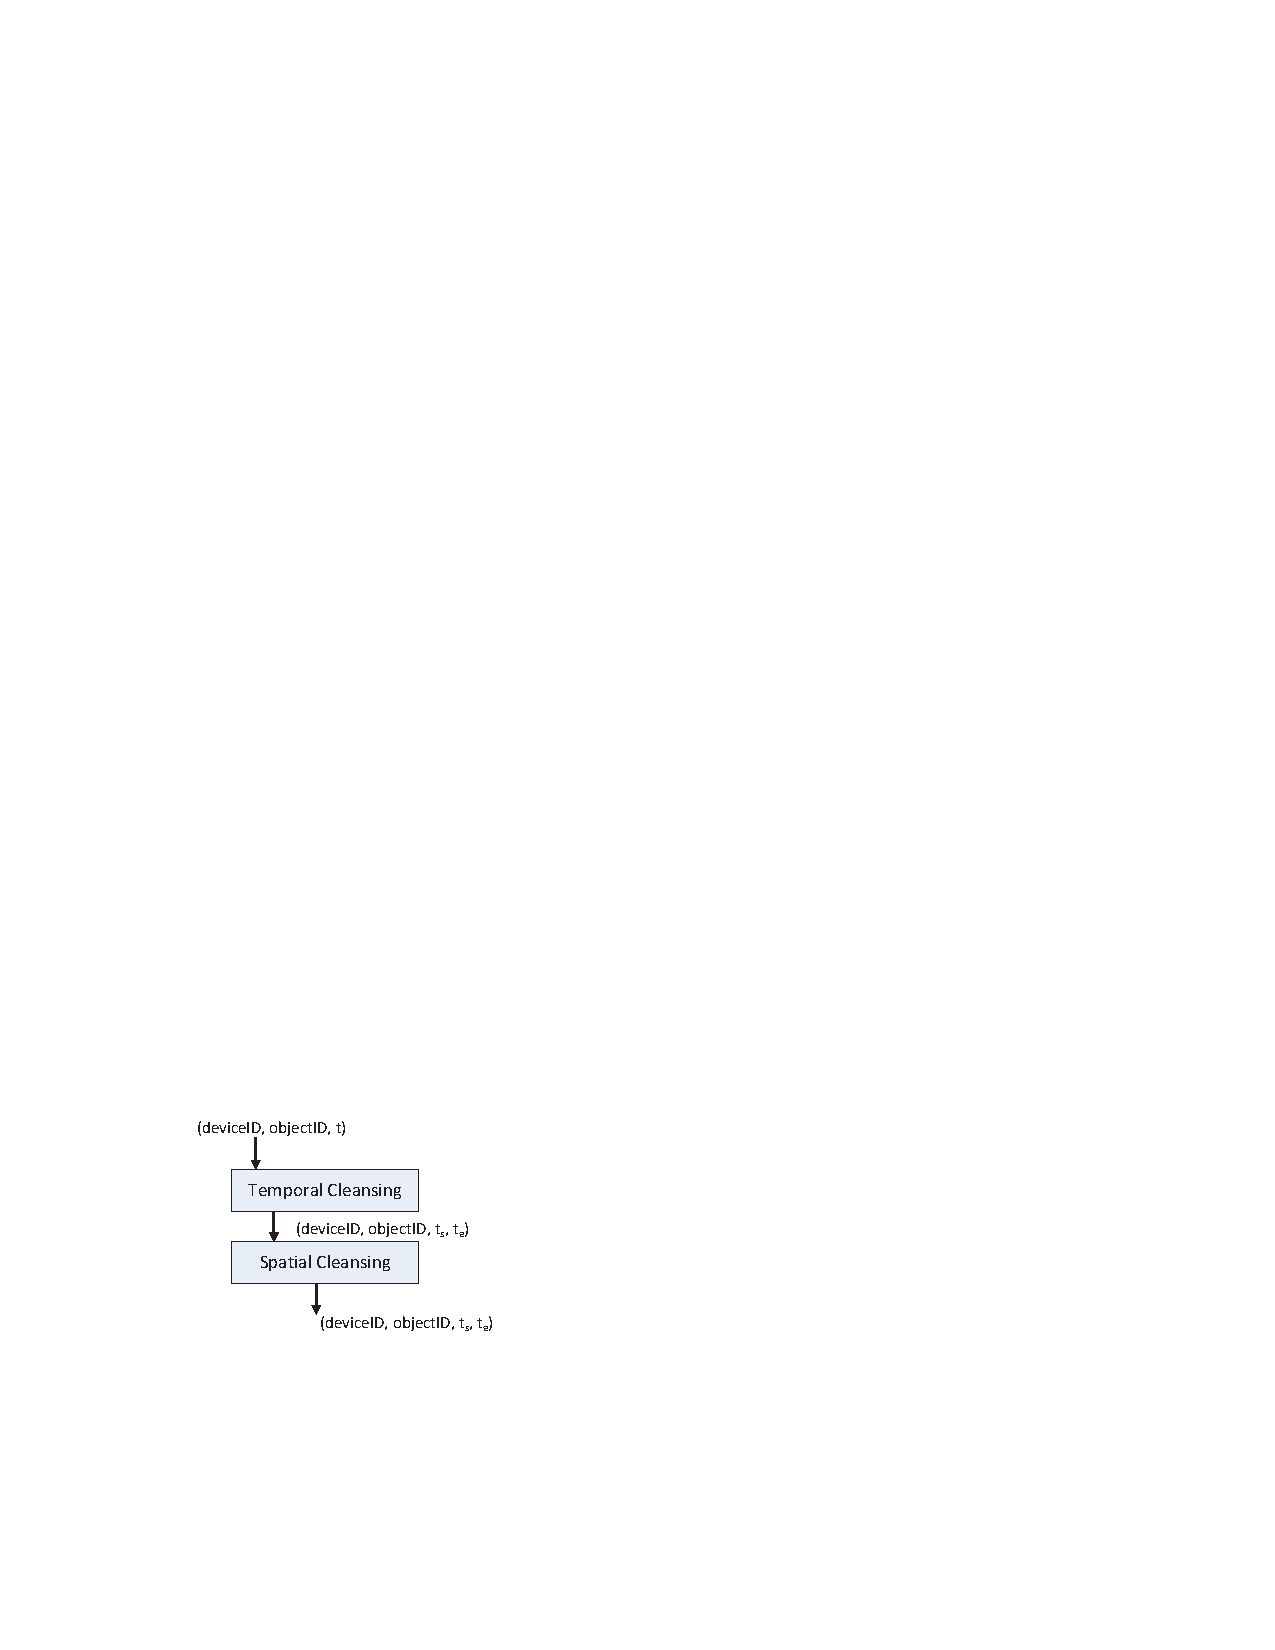
\includegraphics[width=\columnwidth]{figures/3-2/3-2-4.pdf}
\end{figure}

\end{frame}

%------------------------------------------------

\begin{frame}
\frametitle{Phase 1: Temporal Cleansing}

\begin{columns}[c]

  \column{0.5\textwidth}
  \begin{figure}[tb]
    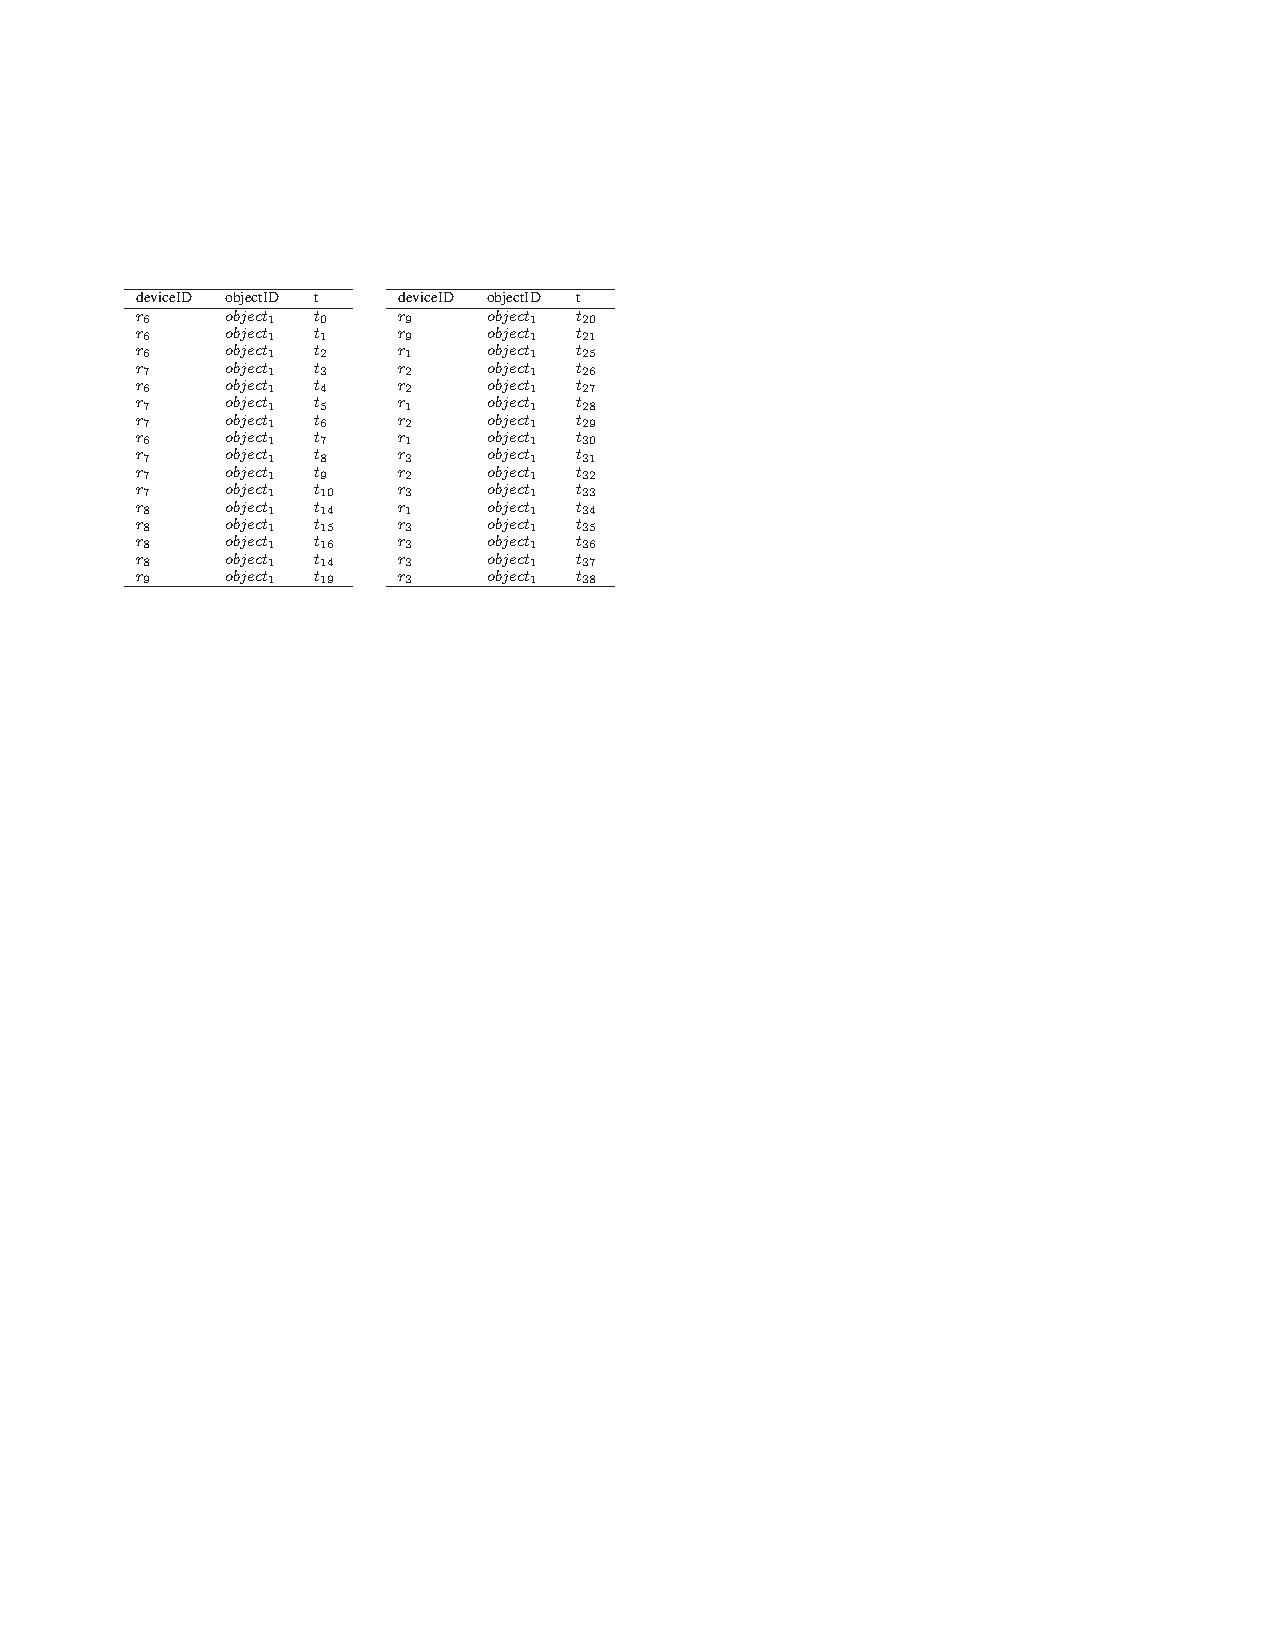
\includegraphics[width=\columnwidth]{figures/3-2/3-2-2.pdf}
  \end{figure}

  \column{0.5\textwidth}
  \begin{figure}[tb]
    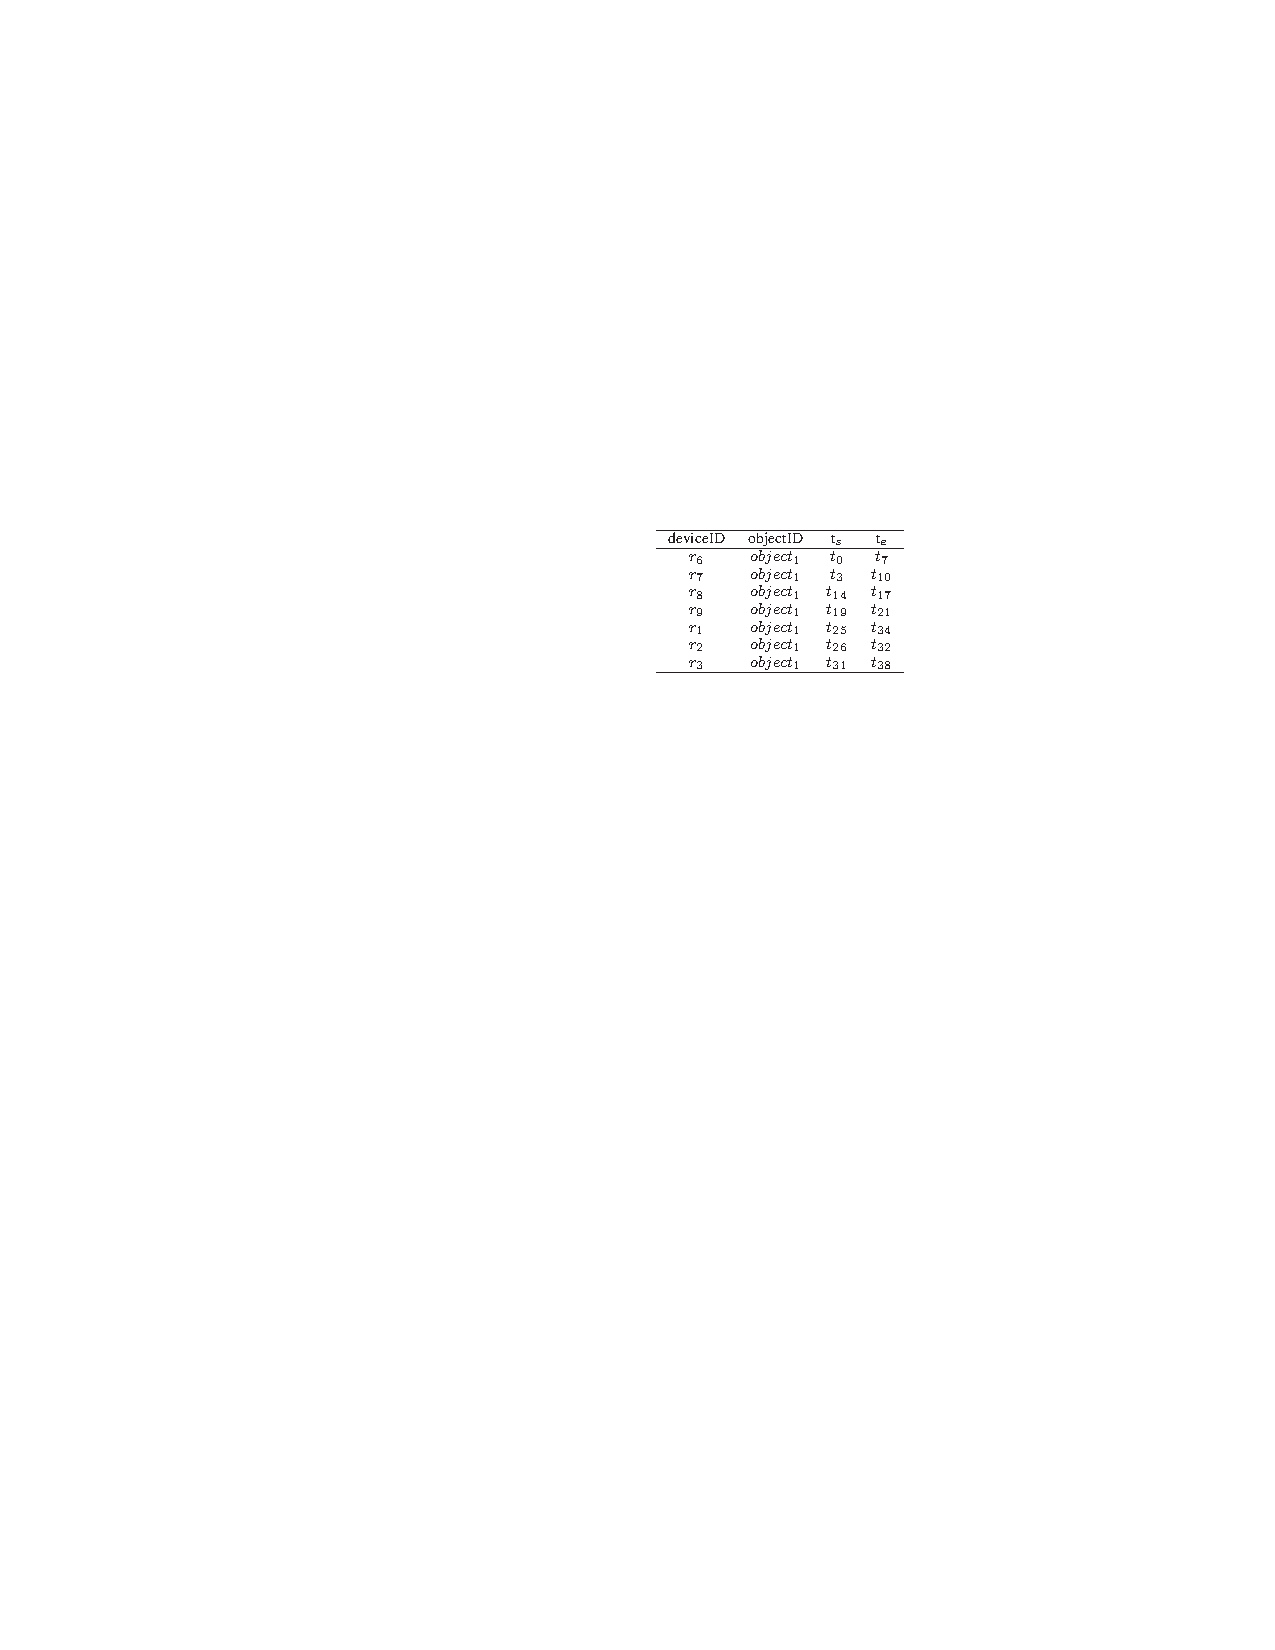
\includegraphics[width=\columnwidth]{figures/3-2/3-2-5.pdf}
  \end{figure}

\end{columns}

\vspace{15pt}
\begin{sitemize}
  \item sequentially scan data from the raw reading table and generates more meaningful tracking records by aggregating on the time.
  \item the aggregation results are controlled by the threshold $\tau$.
  \item all generated tracking records are stored in the \conceptbf{Aggregate Tracking Table} (ATT).
  \item the threshold $\tau$ in the example is 4 time units.
\end{sitemize}

\end{frame}

%------------------------------------------------

\begin{frame}
\frametitle{Phase 2: Spatial Cleansing}

\begin{columns}[c]

  \column{0.5\textwidth}
  \begin{figure}[tb]
    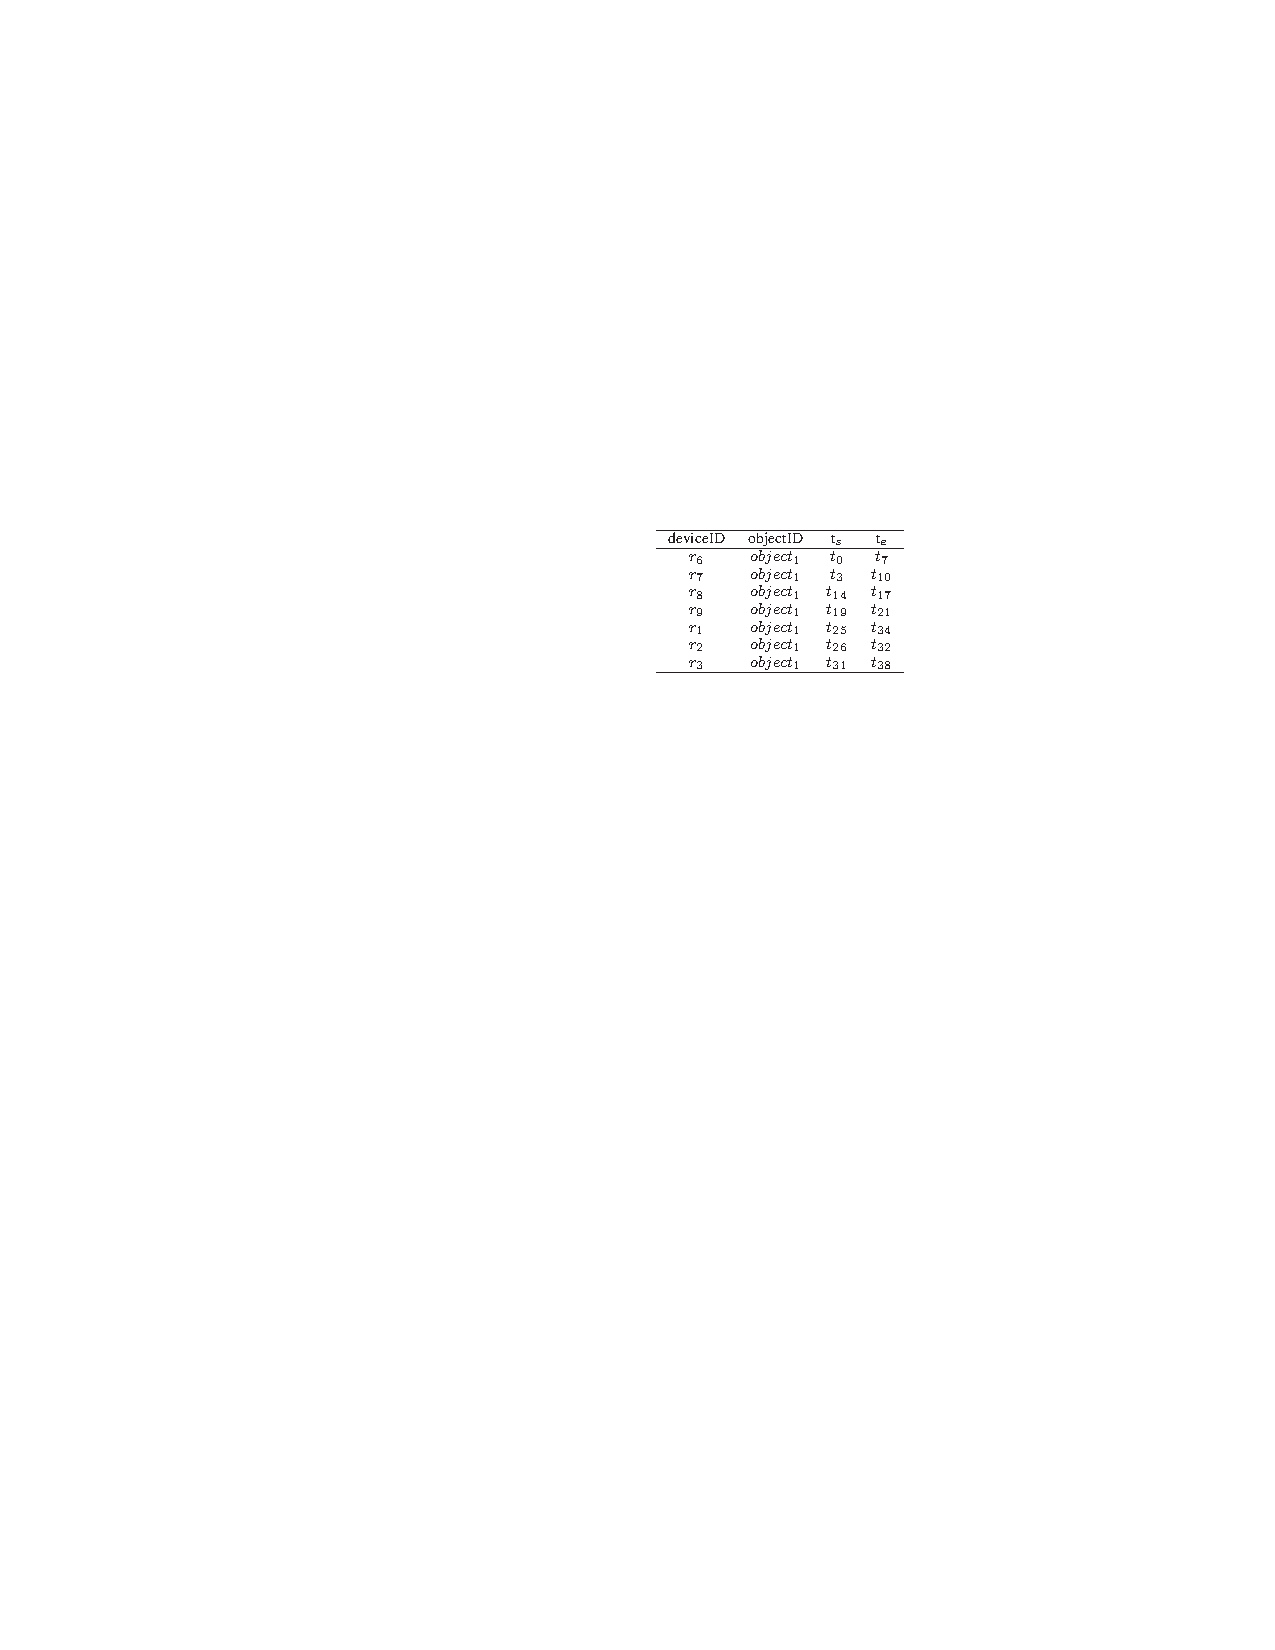
\includegraphics[width=\columnwidth]{figures/3-2/3-2-5.pdf}
  \end{figure}

  \column{0.5\textwidth}
  \begin{figure}[tb]
    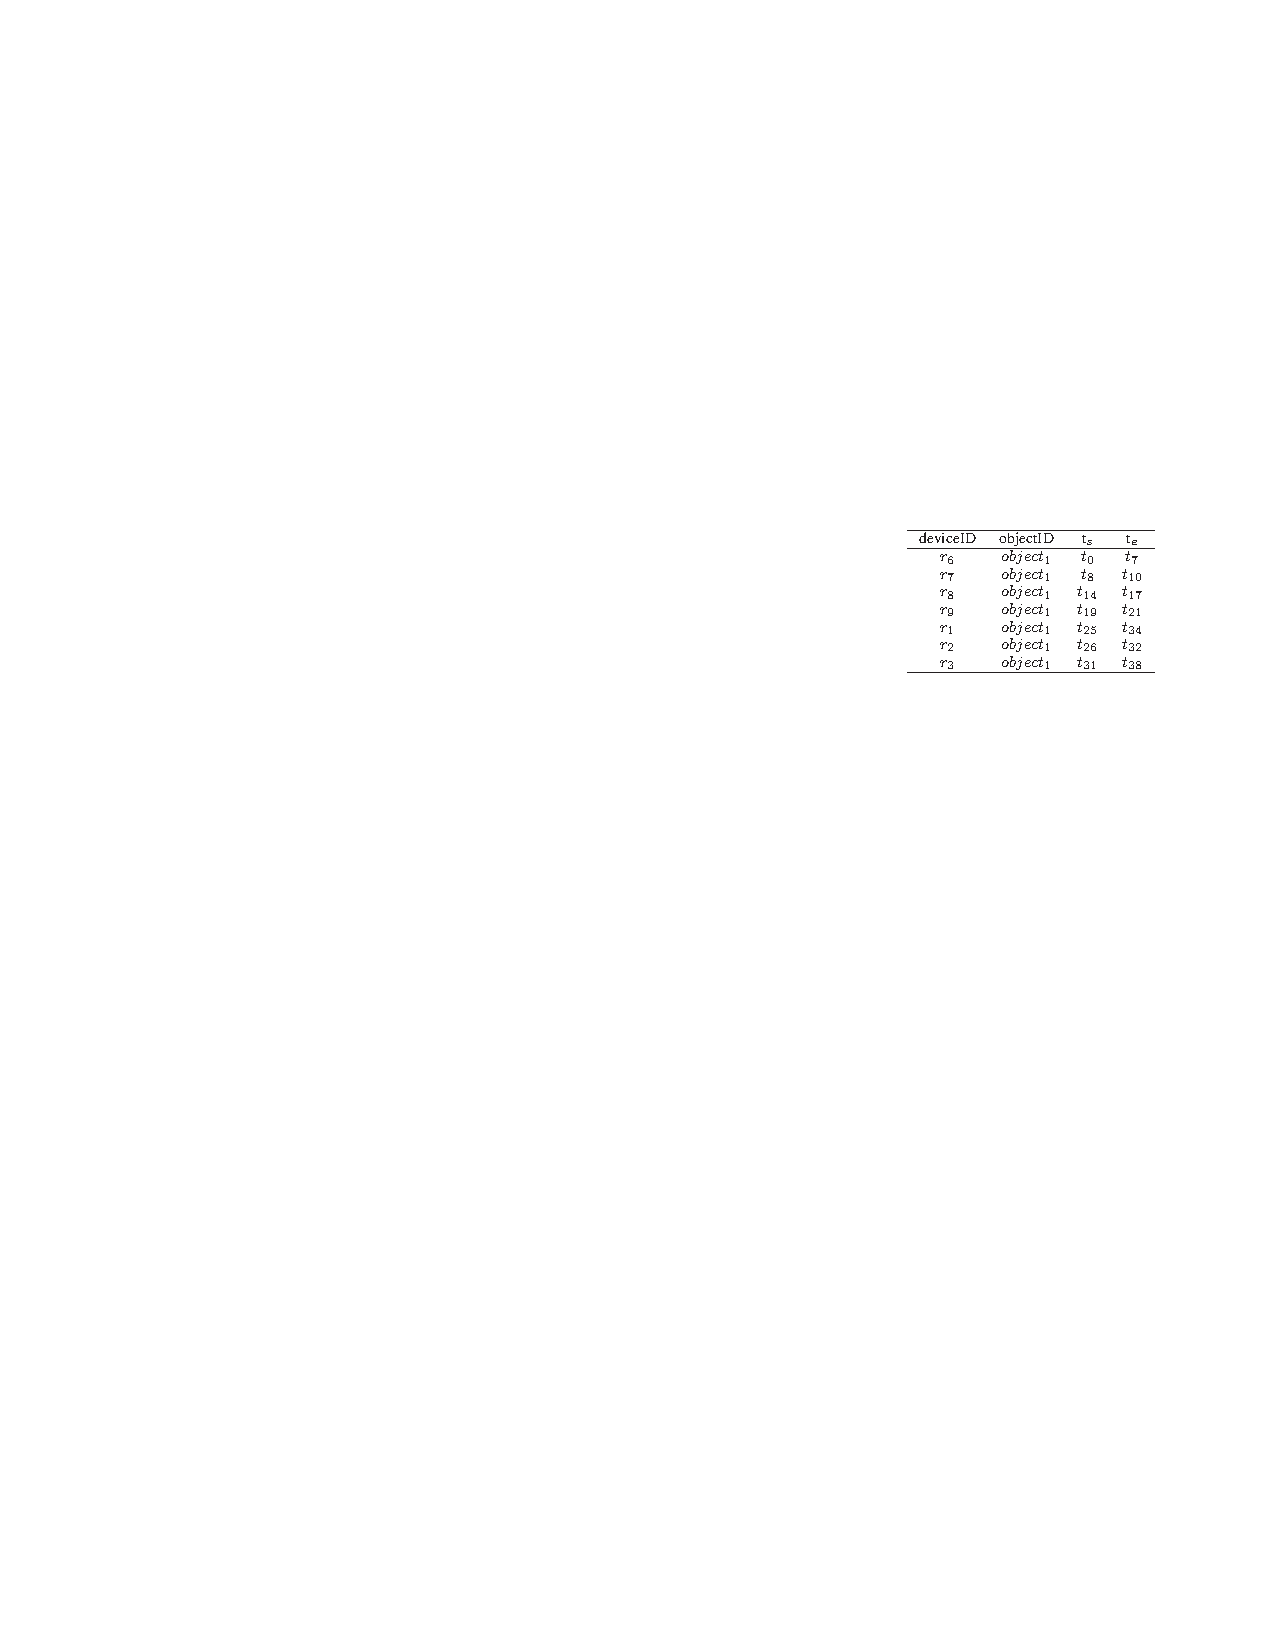
\includegraphics[width=\columnwidth]{figures/3-2/3-2-6.pdf}
  \end{figure}

\end{columns}

\vspace{10pt}
\begin{sitemize}
  \item take the aggregate tracking table as input, identify possible spatial ambiguities, and reduce them by a distance-aware graph.
  \item the distance-aware graph is constructed by all positioning devices in the indoor space.
  \item assuming the minimum movement time between device $r_6$ and $r_7$ is one unit, $object_1$'s tracking record $(r_7, object_1, t_3, t_{10})$ is truncated to $(t_7, object_1, t_8, t_{10})$.
  \item it assumes that the first tracking record in $ATT$ is correct, while it is not always true in practice.
\end{sitemize}

\end{frame}

%------------------------------------------------

\begin{frame}
\frametitle{Temporal Cleansing Algorithm}

\begin{columns}[c]

  \column{0.5\textwidth}
  \begin{figure}[tb]
    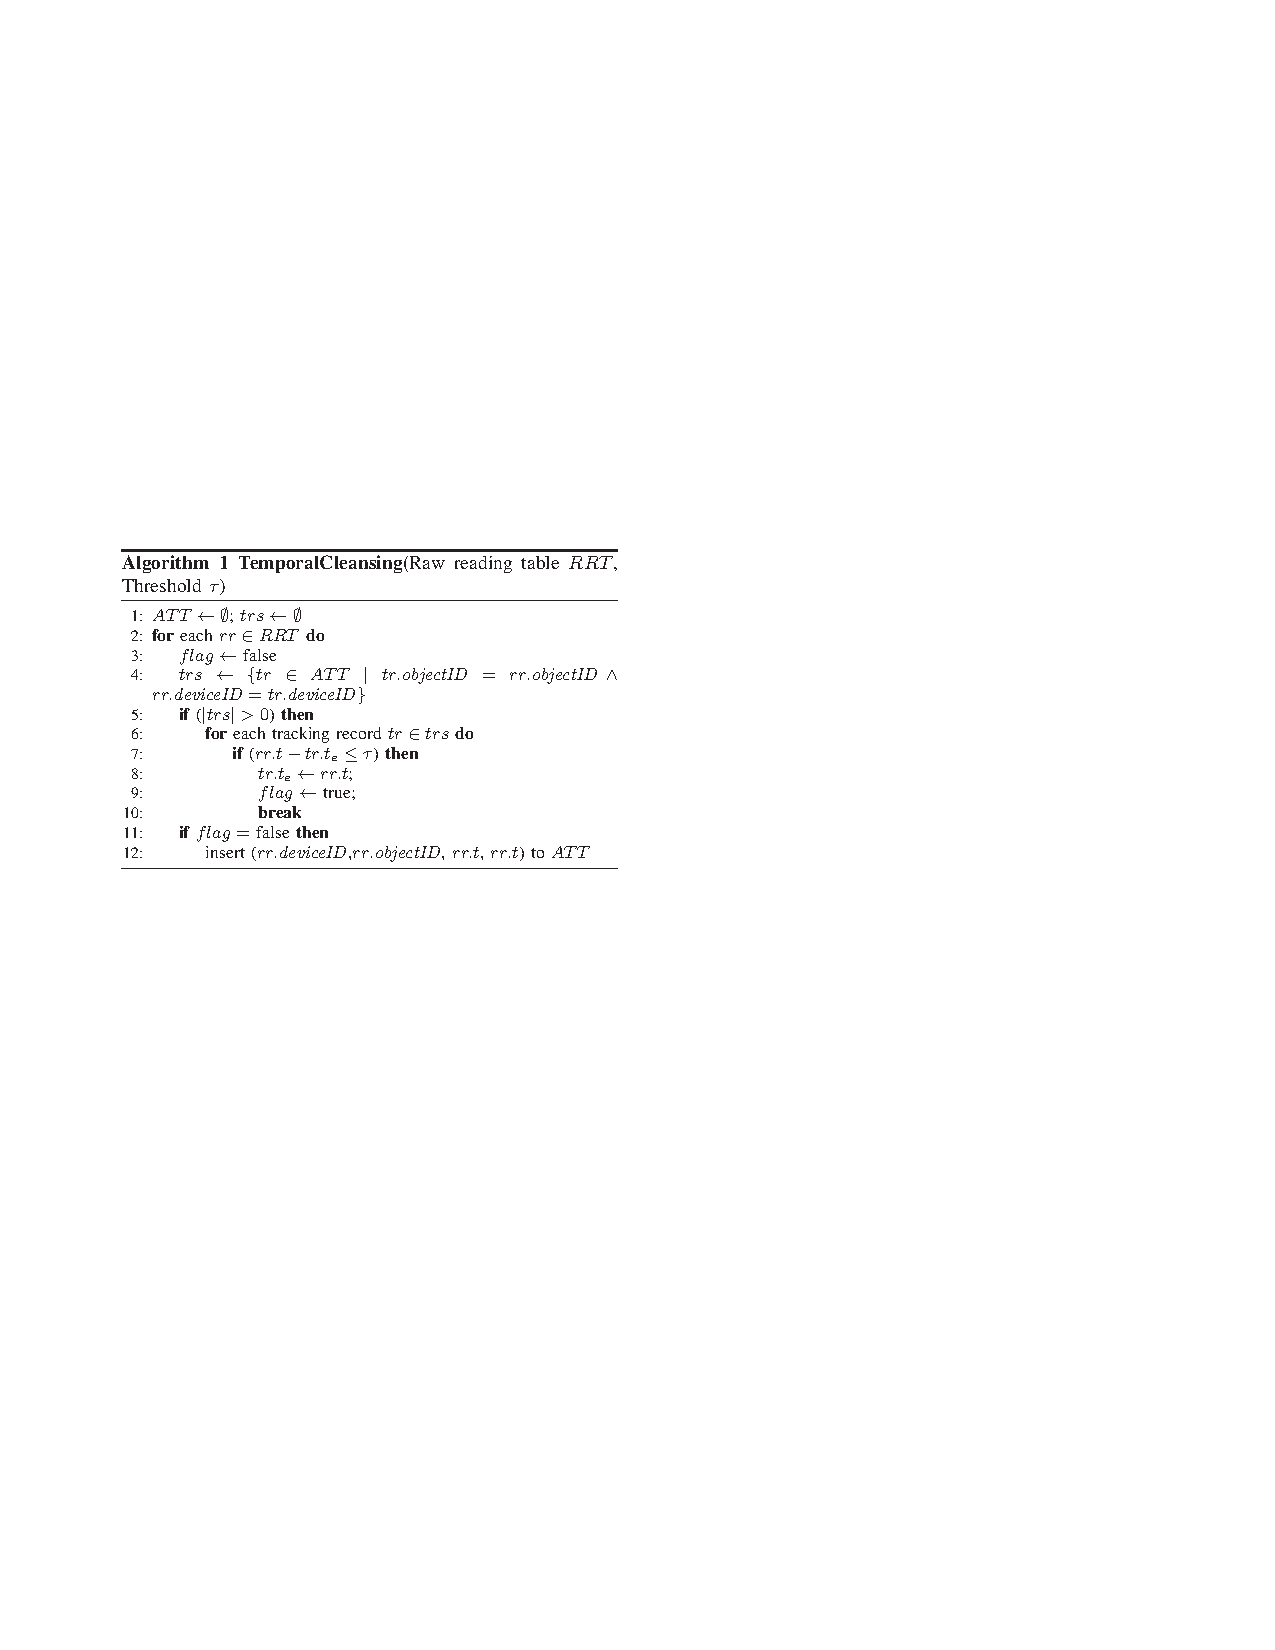
\includegraphics[width=\columnwidth]{figures/3-2/3-2-7.pdf}
  \end{figure}

  \column{0.5\textwidth}
  \begin{sitemize}
    \item Line 1: starts with the initialization of a new aggregate tracking table $ATT$.
    \item Line 4: for each raw reading $rr$ from $RRT$, all the aggregate tracking records with the same device and object as $rr$ in the current $ATT$ are fetched into set $trs$.
    \item Line 5--10: if $trs$ is not empty and $rr$ is temporally close enough to an existing tracking record $tr$ in $trs$, $tr$'s time interval is extended to $rr.t$ and $rr$ is processed.
    \item Line 11--12: otherwise, $rr$ cannot be combined to any existing tracking record, and therefore a new tracking record is created and inserted.
  \end{sitemize}

\end{columns}

\end{frame}

%------------------------------------------------

\begin{frame}
\frametitle{Temporal Cleansing Algorithm: Threshold Setting}

\begin{equation}
  Threshold(\tau) = \frac{\text{detection range diameter}}{\text{object moving speed}}
\end{equation}

\begin{figure}[tb]
  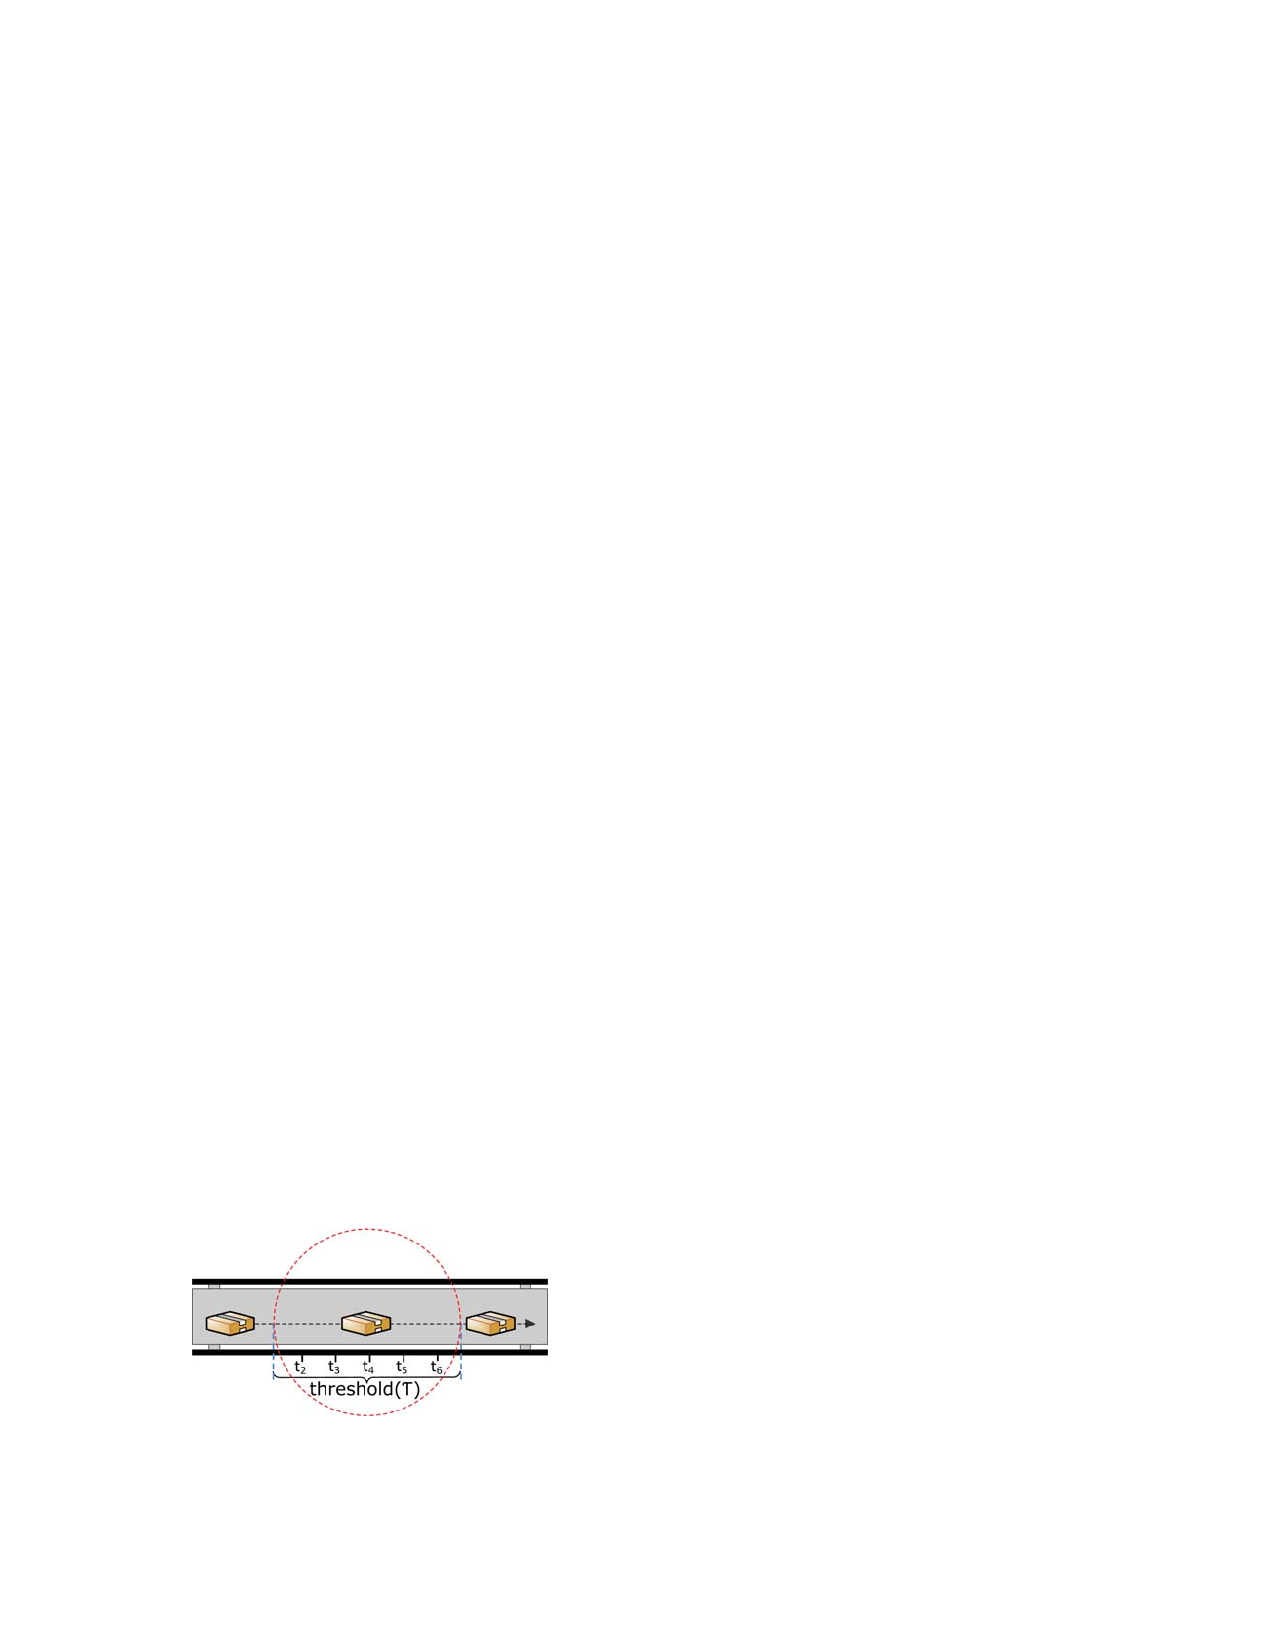
\includegraphics[width=0.7\columnwidth]{figures/3-2/3-2-8.pdf}
\end{figure}

\end{frame}

%------------------------------------------------

\begin{frame}
\frametitle{Distance-Aware Deployment Graph}

\begin{columns}[c]

  \column{0.62\textwidth}
  \ssize{
  \begin{block}{Distance-Aware Deployment Graph}
    $G_{dd} = (V,E,\mathcal{L}_V,\mathcal{L}_E)$
    \begin{sitemize}
      \item $V$ is a set of vertices, each vertex represents a deployed positioning device $r_i$;
      \item $E$ is the set of edges, where $E = \{ (r_i, r_j) | r_i, r_j \in V \wedge r_i \neq r_j \wedge D2V(r_i) \cap D2V(r_j) \neq \varnothing \}$;
      \item $\mathcal{L}_V : V \rightarrow R$ assigns to a vertex $v_i$ the minimum dwell time that an object $o$ should spend in device $r_i$'s detection range such that $o$ is detected by device $r_i$;
      \item $\mathcal{L}_E : E \rightarrow R \times R $ assigns to a edge $(r_i, r_j)$ the minimum indoor walking distance between two devices $r_i$ and $r_j$ and the maximum speed with which an object can move between them, i.e., $\mathcal{L}_E((r_i,r_j)) = (d_{i,j}, S_{i,j})$.
    \end{sitemize}
  \end{block}
  }

  \column{0.38\textwidth}
  \begin{figure}[tb]
    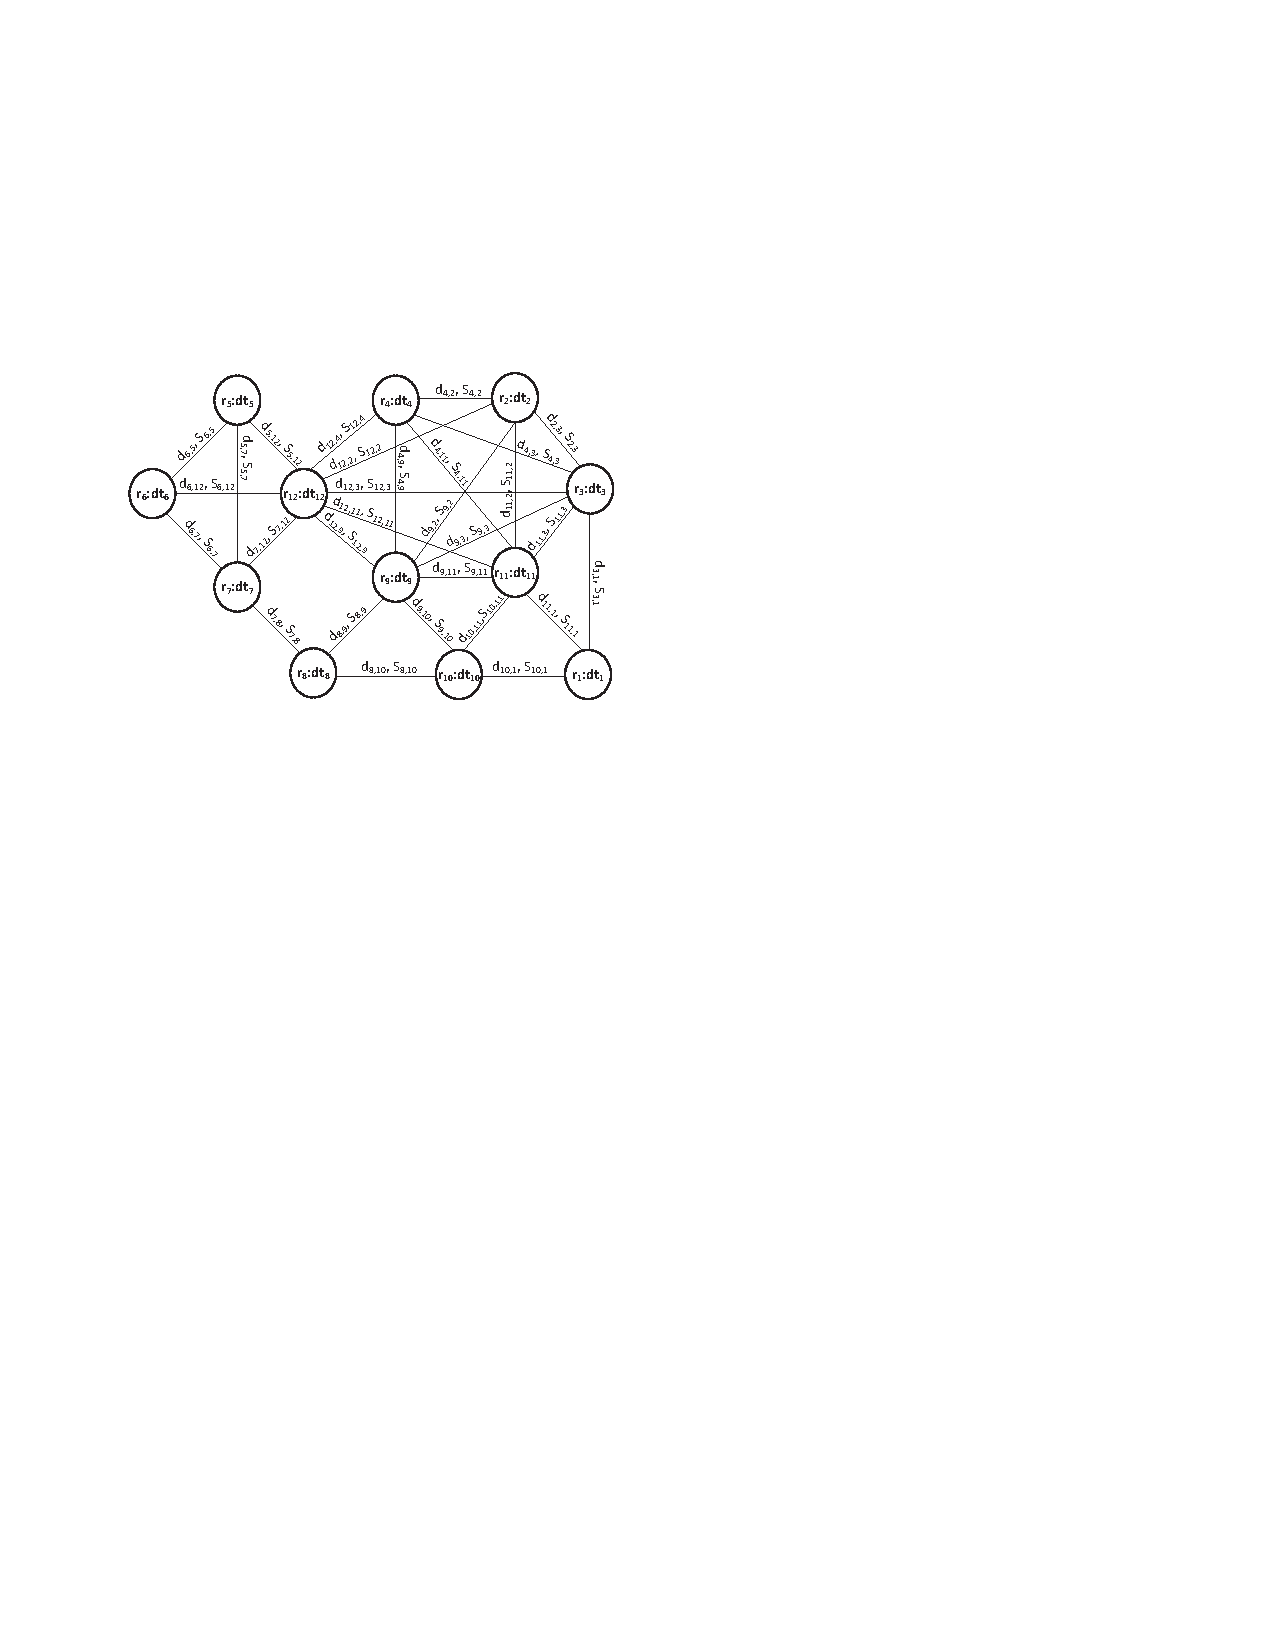
\includegraphics[width=\columnwidth]{figures/3-2/3-2-9.pdf}
  \end{figure}
  \ssize{\textrm{The goal of \emph{Distance-Aware Deployment Graph} is to enable deriving the minimum travel time from one reader to another.}}

\end{columns}

\end{frame}

%------------------------------------------------

\begin{frame}
\frametitle{Distance-Aware Deployment Graph Construction}

\begin{columns}[c]

  \column{0.5\textwidth}
  \begin{figure}[tb]
    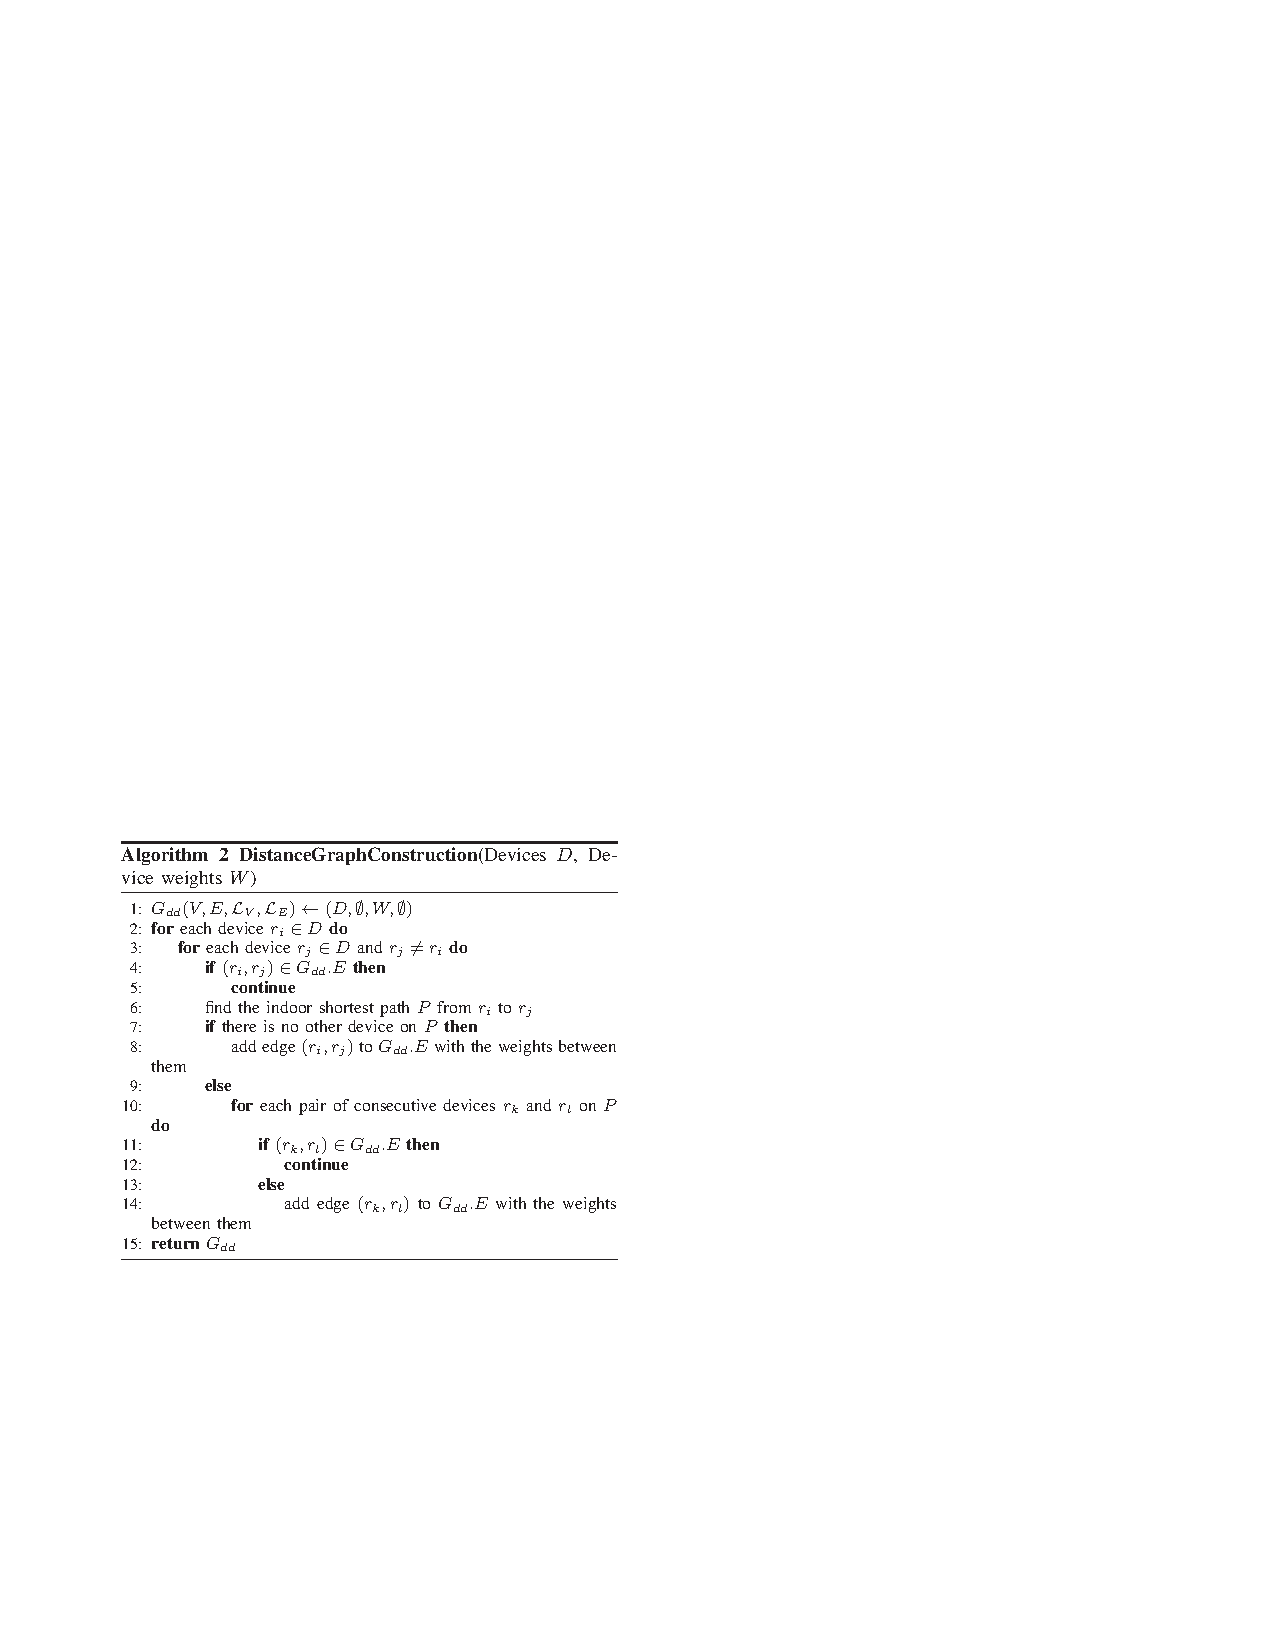
\includegraphics[width=\columnwidth]{figures/3-2/3-2-10.pdf}
  \end{figure}

  \column{0.5\textwidth}
  \begin{sitemize}
    \item Lines 2--6: for each pair of device $r_i$ and $r_j$, the indoor shortest path $P$ is found if the edge $(r_i, r_j)$ is not in the graph yet;
    \item Lines 7--8: if $P$ only contains devices $r_i$ and $r_j$, a new edge is created with the corresponding weights;
    \item Lines 10--14: otherwise each pair of consecutive devices on $P$ are processed likewise.
  \end{sitemize}

\end{columns}

\end{frame}

%------------------------------------------------

\begin{frame}
\frametitle{Spatial Cleansing Algorithm}

\begin{columns}[c]

  \column{0.5\textwidth}
  \begin{figure}[tb]
    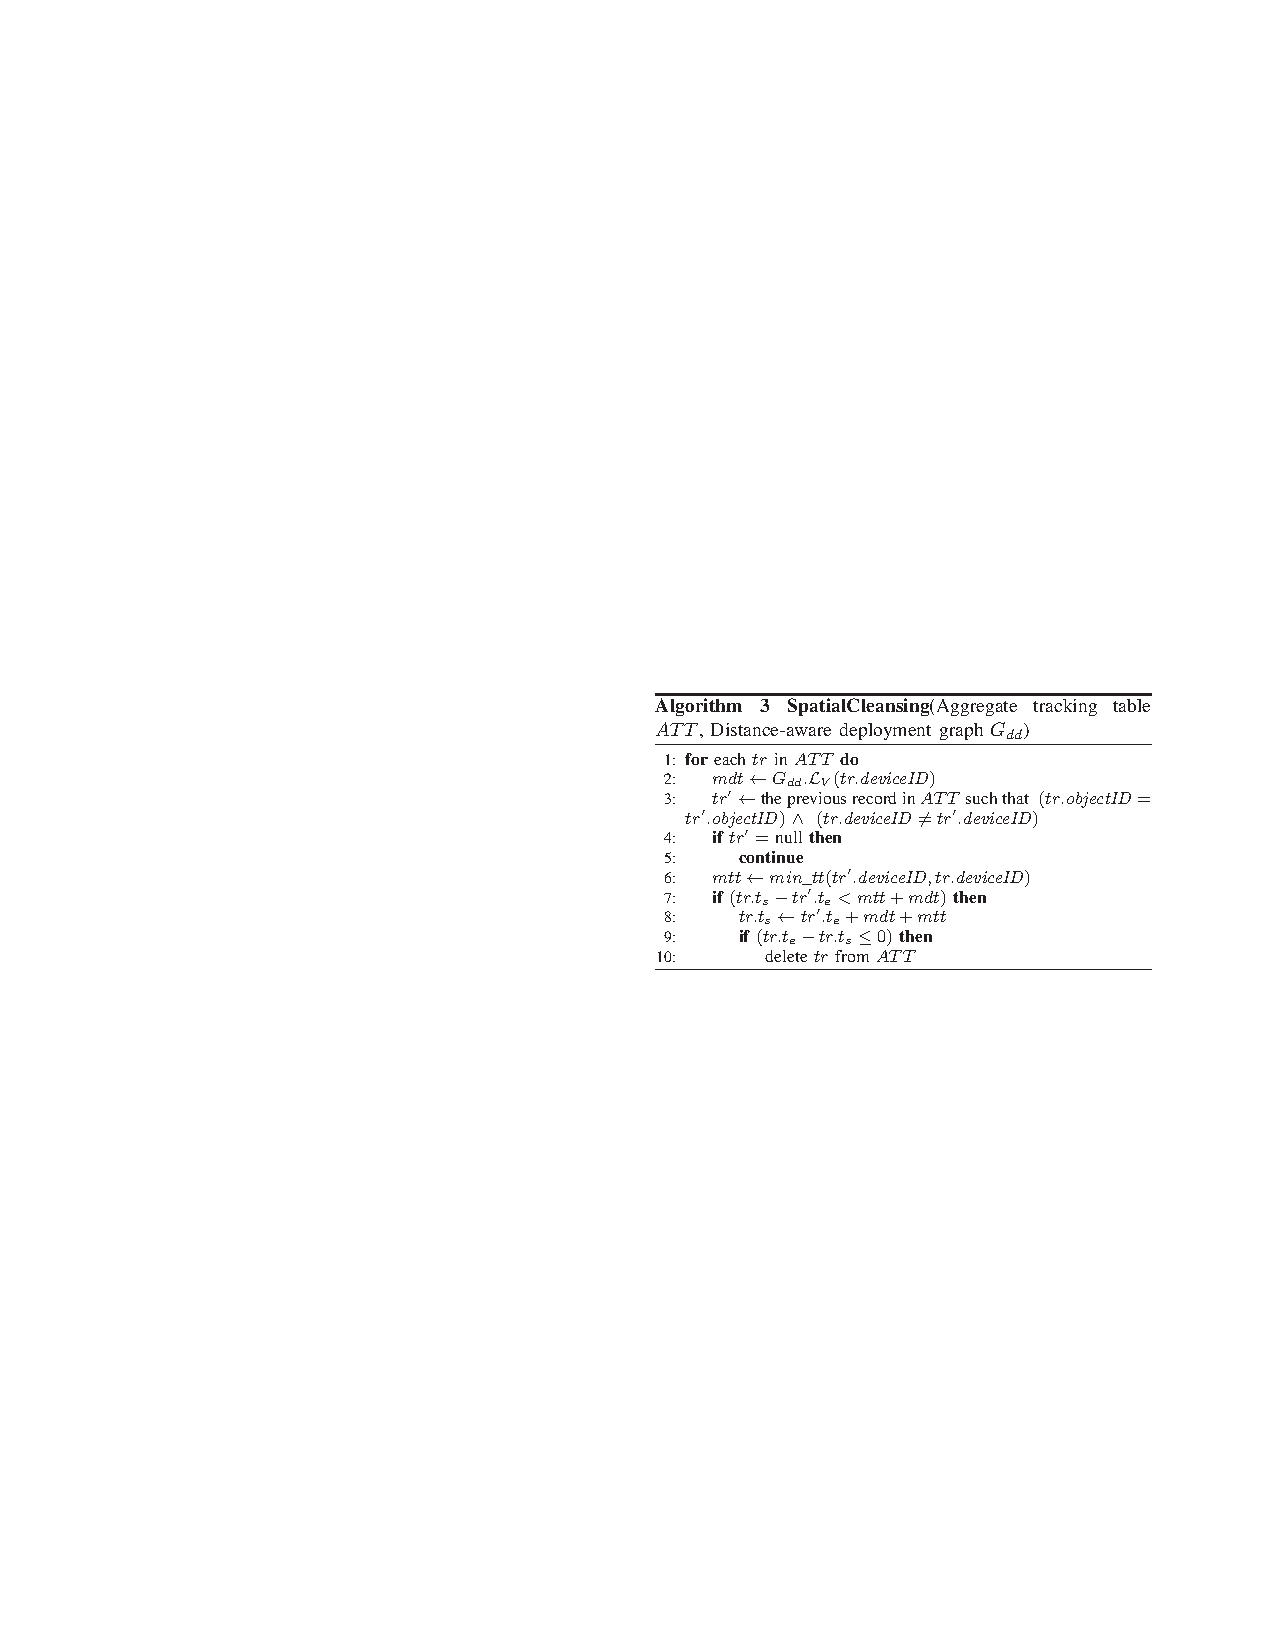
\includegraphics[width=\columnwidth]{figures/3-2/3-2-11.pdf}
  \end{figure}
  \ssize{
  \textrm{
  To identify and reduce the possible spatial ambiguity involving two RFID readers $r_s$ and $r_t$, one should first compute the minimum traveling time $(min\_tt(r_s, r_t))$ that a moving object needs to reach from $r_s$ to $r_t$.
  }
  }

  \column{0.5\textwidth}
  \begin{sitemize}
    \item Line 2: for each tracking record $tr$ in $ATT$, check its dwell time $tr.t_e - tr.t_s$;
    \item Line 3: get $tr$'s previous tracking record $tr'$ from $ATT$ that involves the same object and device as $tr$;
    \item Line 6: get the minimum traveling time from $tr'.deviceID$ and $tr.deviceID$;
    \item Line 7: if the idle time between $tr'$ and $tr$ is too short compared to the minimum traveling time plus the minimum dwell time for $tr.deviceID$;
    \item Line 8: truncate $tr.t_s$ accordingly to make sure the idle time is sufficient with respect to the spatiotemporal constraints;
    \item Lines 9--10: delete $tr$ from $ATT$ if its updated dwell time is too short.
  \end{sitemize}

\end{columns}

\end{frame}

%------------------------------------------------

\begin{frame}
\frametitle{Cases of Spatial Cleansing}

\begin{figure}[tb]
  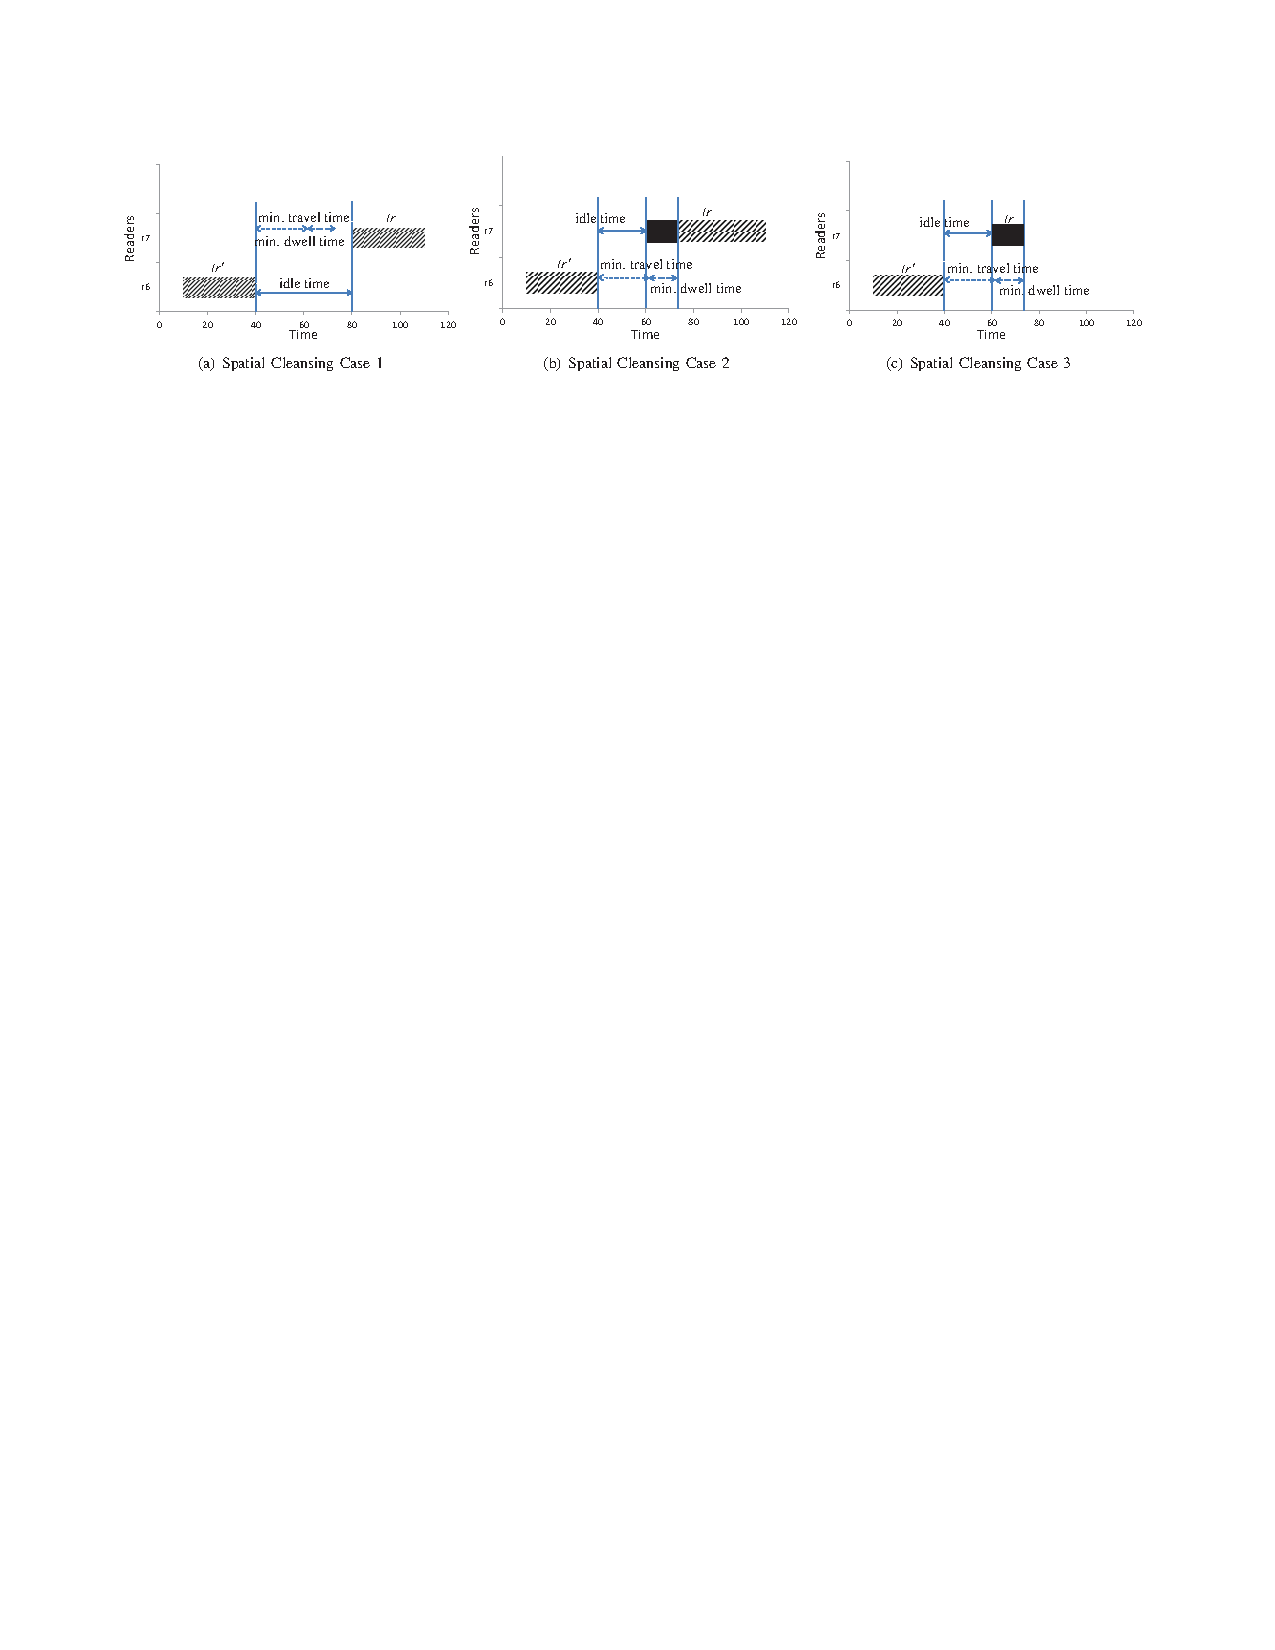
\includegraphics[width=\columnwidth]{figures/3-2/3-2-12.pdf}
\end{figure}

\begin{sitemize}
  \item Case(a): the idle time between two consecutive tracking records is sufficiently long, i.e., longer than the minimum traveling time between devices $r_6$ and $r_7$;
  \item Case(b): it is need to truncate $tr.[t_s, t_e]$, cutting $tr$'s part shown in black, because the idle time between $tr'$ and $tr$ is too short;
  \item Case(c): $tr$ is deleted after the spatial cleansing because its remaining dwell time is too short.
\end{sitemize}

\end{frame}

%------------------------------------------------

\begin{frame}
\frametitle{Conclusions}



It designs a temporal cleansing algorithm to aggregate raw RFID readings temporally such that the data size is compressed without information loss.\\~\\

It designs a spatial cleansing technique: proposing a distance-aware deployment graph to capture the spatiotemporal constrains implied by the deployment of RFID readers as well as the indoor topology.\\~\\

The techniques proposed in this paper also apply to indoor tracking data obtained by other symbolic positioning technologies, like Bluetooth.


\end{frame}
